\documentclass[xcolor=table]{beamer}

\usepackage{booktabs}
\usepackage{hyperref}
\usepackage[table]{xcolor}
\usepackage{tikz}
\usepackage{graphics}
\usetikzlibrary{calc}

\setbeamertemplate{navigation symbols}{}%remove navigation symbols

\title{Population Games}
\subtitle{Game Theory}
\author{Vincent Knight}
\date{}

\begin{document}

\frame{\titlepage}

\frame{
\begin{center}
\begin{tikzpicture}[scale=.5]
\only<1>{\node at (0, 0) [fill, color=black] {};}
\only<2->{\node at (0, 0) [fill, color=red] {};}
\only<1>{\node at (0, 1) [fill, color=black] {};}
\only<2-9>{\node at (0, 1) [fill, color=green] {};}
\only<10->{\node at (0, 1) [fill, color=red] {};}
\only<1>{\node at (0, 2) [fill, color=black] {};}
\only<2-6>{\node at (0, 2) [fill, color=green] {};}
\only<7->{\node at (0, 2) [fill, color=red] {};}
\only<1>{\node at (0, 3) [fill, color=black] {};}
\only<2-7>{\node at (0, 3) [fill, color=green] {};}
\only<8->{\node at (0, 3) [fill, color=red] {};}
\only<1>{\node at (0, 4) [fill, color=black] {};}
\only<2-6>{\node at (0, 4) [fill, color=green] {};}
\only<7->{\node at (0, 4) [fill, color=red] {};}
\only<1>{\node at (0, 5) [fill, color=black] {};}
\only<2-3>{\node at (0, 5) [fill, color=green] {};}
\only<4->{\node at (0, 5) [fill, color=red] {};}
\only<1>{\node at (0, 6) [fill, color=black] {};}
\only<2-4>{\node at (0, 6) [fill, color=green] {};}
\only<5->{\node at (0, 6) [fill, color=red] {};}
\only<1>{\node at (0, 7) [fill, color=black] {};}
\only<2-9>{\node at (0, 7) [fill, color=green] {};}
\only<10->{\node at (0, 7) [fill, color=red] {};}
\only<1>{\node at (0, 8) [fill, color=black] {};}
\only<2->{\node at (0, 8) [fill, color=red] {};}
\only<1>{\node at (0, 9) [fill, color=black] {};}
\only<2-3>{\node at (0, 9) [fill, color=green] {};}
\only<4->{\node at (0, 9) [fill, color=red] {};}
\only<1>{\node at (1, 0) [fill, color=black] {};}
\only<2->{\node at (1, 0) [fill, color=red] {};}
\only<1>{\node at (1, 1) [fill, color=black] {};}
\only<2-9>{\node at (1, 1) [fill, color=green] {};}
\only<10->{\node at (1, 1) [fill, color=red] {};}
\only<1>{\node at (1, 2) [fill, color=black] {};}
\only<2->{\node at (1, 2) [fill, color=red] {};}
\only<1>{\node at (1, 3) [fill, color=black] {};}
\only<2-8>{\node at (1, 3) [fill, color=green] {};}
\only<9->{\node at (1, 3) [fill, color=red] {};}
\only<1>{\node at (1, 4) [fill, color=black] {};}
\only<2->{\node at (1, 4) [fill, color=red] {};}
\only<1>{\node at (1, 5) [fill, color=black] {};}
\only<2-2>{\node at (1, 5) [fill, color=green] {};}
\only<3->{\node at (1, 5) [fill, color=red] {};}
\only<1>{\node at (1, 6) [fill, color=black] {};}
\only<2-6>{\node at (1, 6) [fill, color=green] {};}
\only<7->{\node at (1, 6) [fill, color=red] {};}
\only<1>{\node at (1, 7) [fill, color=black] {};}
\only<2-4>{\node at (1, 7) [fill, color=green] {};}
\only<5->{\node at (1, 7) [fill, color=red] {};}
\only<1>{\node at (1, 8) [fill, color=black] {};}
\only<2->{\node at (1, 8) [fill, color=red] {};}
\only<1>{\node at (1, 9) [fill, color=black] {};}
\only<2-2>{\node at (1, 9) [fill, color=green] {};}
\only<3->{\node at (1, 9) [fill, color=red] {};}
\only<1>{\node at (2, 0) [fill, color=black] {};}
\only<2-2>{\node at (2, 0) [fill, color=green] {};}
\only<3->{\node at (2, 0) [fill, color=red] {};}
\only<1>{\node at (2, 1) [fill, color=black] {};}
\only<2-7>{\node at (2, 1) [fill, color=green] {};}
\only<8->{\node at (2, 1) [fill, color=red] {};}
\only<1>{\node at (2, 2) [fill, color=black] {};}
\only<2-2>{\node at (2, 2) [fill, color=green] {};}
\only<3->{\node at (2, 2) [fill, color=red] {};}
\only<1>{\node at (2, 3) [fill, color=black] {};}
\only<2->{\node at (2, 3) [fill, color=red] {};}
\only<1>{\node at (2, 4) [fill, color=black] {};}
\only<2-4>{\node at (2, 4) [fill, color=green] {};}
\only<5->{\node at (2, 4) [fill, color=red] {};}
\only<1>{\node at (2, 5) [fill, color=black] {};}
\only<2-4>{\node at (2, 5) [fill, color=green] {};}
\only<5->{\node at (2, 5) [fill, color=red] {};}
\only<1>{\node at (2, 6) [fill, color=black] {};}
\only<2-8>{\node at (2, 6) [fill, color=green] {};}
\only<9->{\node at (2, 6) [fill, color=red] {};}
\only<1>{\node at (2, 7) [fill, color=black] {};}
\only<2-9>{\node at (2, 7) [fill, color=green] {};}
\only<10->{\node at (2, 7) [fill, color=red] {};}
\only<1>{\node at (2, 8) [fill, color=black] {};}
\only<2-6>{\node at (2, 8) [fill, color=green] {};}
\only<7->{\node at (2, 8) [fill, color=red] {};}
\only<1>{\node at (2, 9) [fill, color=black] {};}
\only<2-7>{\node at (2, 9) [fill, color=green] {};}
\only<8->{\node at (2, 9) [fill, color=red] {};}
\only<1>{\node at (3, 0) [fill, color=black] {};}
\only<2-8>{\node at (3, 0) [fill, color=green] {};}
\only<9->{\node at (3, 0) [fill, color=red] {};}
\only<1>{\node at (3, 1) [fill, color=black] {};}
\only<2-8>{\node at (3, 1) [fill, color=green] {};}
\only<9->{\node at (3, 1) [fill, color=red] {};}
\only<1>{\node at (3, 2) [fill, color=black] {};}
\only<2-6>{\node at (3, 2) [fill, color=green] {};}
\only<7->{\node at (3, 2) [fill, color=red] {};}
\only<1>{\node at (3, 3) [fill, color=black] {};}
\only<2->{\node at (3, 3) [fill, color=red] {};}
\only<1>{\node at (3, 4) [fill, color=black] {};}
\only<2->{\node at (3, 4) [fill, color=red] {};}
\only<1>{\node at (3, 5) [fill, color=black] {};}
\only<2-3>{\node at (3, 5) [fill, color=green] {};}
\only<4->{\node at (3, 5) [fill, color=red] {};}
\only<1>{\node at (3, 6) [fill, color=black] {};}
\only<2-7>{\node at (3, 6) [fill, color=green] {};}
\only<8->{\node at (3, 6) [fill, color=red] {};}
\only<1>{\node at (3, 7) [fill, color=black] {};}
\only<2-9>{\node at (3, 7) [fill, color=green] {};}
\only<10->{\node at (3, 7) [fill, color=red] {};}
\only<1>{\node at (3, 8) [fill, color=black] {};}
\only<2-4>{\node at (3, 8) [fill, color=green] {};}
\only<5->{\node at (3, 8) [fill, color=red] {};}
\only<1>{\node at (3, 9) [fill, color=black] {};}
\only<2-4>{\node at (3, 9) [fill, color=green] {};}
\only<5->{\node at (3, 9) [fill, color=red] {};}
\only<1>{\node at (4, 0) [fill, color=black] {};}
\only<2-5>{\node at (4, 0) [fill, color=green] {};}
\only<6->{\node at (4, 0) [fill, color=red] {};}
\only<1>{\node at (4, 1) [fill, color=black] {};}
\only<2->{\node at (4, 1) [fill, color=red] {};}
\only<1>{\node at (4, 2) [fill, color=black] {};}
\only<2-5>{\node at (4, 2) [fill, color=green] {};}
\only<6->{\node at (4, 2) [fill, color=red] {};}
\only<1>{\node at (4, 3) [fill, color=black] {};}
\only<2->{\node at (4, 3) [fill, color=red] {};}
\only<1>{\node at (4, 4) [fill, color=black] {};}
\only<2-8>{\node at (4, 4) [fill, color=green] {};}
\only<9->{\node at (4, 4) [fill, color=red] {};}
\only<1>{\node at (4, 5) [fill, color=black] {};}
\only<2-6>{\node at (4, 5) [fill, color=green] {};}
\only<7->{\node at (4, 5) [fill, color=red] {};}
\only<1>{\node at (4, 6) [fill, color=black] {};}
\only<2-5>{\node at (4, 6) [fill, color=green] {};}
\only<6->{\node at (4, 6) [fill, color=red] {};}
\only<1>{\node at (4, 7) [fill, color=black] {};}
\only<2-2>{\node at (4, 7) [fill, color=green] {};}
\only<3->{\node at (4, 7) [fill, color=red] {};}
\only<1>{\node at (4, 8) [fill, color=black] {};}
\only<2-4>{\node at (4, 8) [fill, color=green] {};}
\only<5->{\node at (4, 8) [fill, color=red] {};}
\only<1>{\node at (4, 9) [fill, color=black] {};}
\only<2->{\node at (4, 9) [fill, color=red] {};}
\only<1>{\node at (5, 0) [fill, color=black] {};}
\only<2-7>{\node at (5, 0) [fill, color=green] {};}
\only<8->{\node at (5, 0) [fill, color=red] {};}
\only<1>{\node at (5, 1) [fill, color=black] {};}
\only<2-3>{\node at (5, 1) [fill, color=green] {};}
\only<4->{\node at (5, 1) [fill, color=red] {};}
\only<1>{\node at (5, 2) [fill, color=black] {};}
\only<2-4>{\node at (5, 2) [fill, color=green] {};}
\only<5->{\node at (5, 2) [fill, color=red] {};}
\only<1>{\node at (5, 3) [fill, color=black] {};}
\only<2-8>{\node at (5, 3) [fill, color=green] {};}
\only<9->{\node at (5, 3) [fill, color=red] {};}
\only<1>{\node at (5, 4) [fill, color=black] {};}
\only<2-4>{\node at (5, 4) [fill, color=green] {};}
\only<5->{\node at (5, 4) [fill, color=red] {};}
\only<1>{\node at (5, 5) [fill, color=black] {};}
\only<2-4>{\node at (5, 5) [fill, color=green] {};}
\only<5->{\node at (5, 5) [fill, color=red] {};}
\only<1>{\node at (5, 6) [fill, color=black] {};}
\only<2->{\node at (5, 6) [fill, color=red] {};}
\only<1>{\node at (5, 7) [fill, color=black] {};}
\only<2-4>{\node at (5, 7) [fill, color=green] {};}
\only<5->{\node at (5, 7) [fill, color=red] {};}
\only<1>{\node at (5, 8) [fill, color=black] {};}
\only<2->{\node at (5, 8) [fill, color=red] {};}
\only<1>{\node at (5, 9) [fill, color=black] {};}
\only<2->{\node at (5, 9) [fill, color=red] {};}
\only<1>{\node at (6, 0) [fill, color=black] {};}
\only<2-7>{\node at (6, 0) [fill, color=green] {};}
\only<8->{\node at (6, 0) [fill, color=red] {};}
\only<1>{\node at (6, 1) [fill, color=black] {};}
\only<2-7>{\node at (6, 1) [fill, color=green] {};}
\only<8->{\node at (6, 1) [fill, color=red] {};}
\only<1>{\node at (6, 2) [fill, color=black] {};}
\only<2->{\node at (6, 2) [fill, color=red] {};}
\only<1>{\node at (6, 3) [fill, color=black] {};}
\only<2-6>{\node at (6, 3) [fill, color=green] {};}
\only<7->{\node at (6, 3) [fill, color=red] {};}
\only<1>{\node at (6, 4) [fill, color=black] {};}
\only<2-4>{\node at (6, 4) [fill, color=green] {};}
\only<5->{\node at (6, 4) [fill, color=red] {};}
\only<1>{\node at (6, 5) [fill, color=black] {};}
\only<2-9>{\node at (6, 5) [fill, color=green] {};}
\only<10->{\node at (6, 5) [fill, color=red] {};}
\only<1>{\node at (6, 6) [fill, color=black] {};}
\only<2-9>{\node at (6, 6) [fill, color=green] {};}
\only<10->{\node at (6, 6) [fill, color=red] {};}
\only<1>{\node at (6, 7) [fill, color=black] {};}
\only<2-2>{\node at (6, 7) [fill, color=green] {};}
\only<3->{\node at (6, 7) [fill, color=red] {};}
\only<1>{\node at (6, 8) [fill, color=black] {};}
\only<2-6>{\node at (6, 8) [fill, color=green] {};}
\only<7->{\node at (6, 8) [fill, color=red] {};}
\only<1>{\node at (6, 9) [fill, color=black] {};}
\only<2-8>{\node at (6, 9) [fill, color=green] {};}
\only<9->{\node at (6, 9) [fill, color=red] {};}
\only<1>{\node at (7, 0) [fill, color=black] {};}
\only<2->{\node at (7, 0) [fill, color=red] {};}
\only<1>{\node at (7, 1) [fill, color=black] {};}
\only<2-2>{\node at (7, 1) [fill, color=green] {};}
\only<3->{\node at (7, 1) [fill, color=red] {};}
\only<1>{\node at (7, 2) [fill, color=black] {};}
\only<2-5>{\node at (7, 2) [fill, color=green] {};}
\only<6->{\node at (7, 2) [fill, color=red] {};}
\only<1>{\node at (7, 3) [fill, color=black] {};}
\only<2-9>{\node at (7, 3) [fill, color=green] {};}
\only<10->{\node at (7, 3) [fill, color=red] {};}
\only<1>{\node at (7, 4) [fill, color=black] {};}
\only<2-8>{\node at (7, 4) [fill, color=green] {};}
\only<9->{\node at (7, 4) [fill, color=red] {};}
\only<1>{\node at (7, 5) [fill, color=black] {};}
\only<2-4>{\node at (7, 5) [fill, color=green] {};}
\only<5->{\node at (7, 5) [fill, color=red] {};}
\only<1>{\node at (7, 6) [fill, color=black] {};}
\only<2->{\node at (7, 6) [fill, color=red] {};}
\only<1>{\node at (7, 7) [fill, color=black] {};}
\only<2-2>{\node at (7, 7) [fill, color=green] {};}
\only<3->{\node at (7, 7) [fill, color=red] {};}
\only<1>{\node at (7, 8) [fill, color=black] {};}
\only<2-7>{\node at (7, 8) [fill, color=green] {};}
\only<8->{\node at (7, 8) [fill, color=red] {};}
\only<1>{\node at (7, 9) [fill, color=black] {};}
\only<2-4>{\node at (7, 9) [fill, color=green] {};}
\only<5->{\node at (7, 9) [fill, color=red] {};}
\only<1>{\node at (8, 0) [fill, color=black] {};}
\only<2-6>{\node at (8, 0) [fill, color=green] {};}
\only<7->{\node at (8, 0) [fill, color=red] {};}
\only<1>{\node at (8, 1) [fill, color=black] {};}
\only<2-8>{\node at (8, 1) [fill, color=green] {};}
\only<9->{\node at (8, 1) [fill, color=red] {};}
\only<1>{\node at (8, 2) [fill, color=black] {};}
\only<2-8>{\node at (8, 2) [fill, color=green] {};}
\only<9->{\node at (8, 2) [fill, color=red] {};}
\only<1>{\node at (8, 3) [fill, color=black] {};}
\only<2-7>{\node at (8, 3) [fill, color=green] {};}
\only<8->{\node at (8, 3) [fill, color=red] {};}
\only<1>{\node at (8, 4) [fill, color=black] {};}
\only<2->{\node at (8, 4) [fill, color=red] {};}
\only<1>{\node at (8, 5) [fill, color=black] {};}
\only<2-4>{\node at (8, 5) [fill, color=green] {};}
\only<5->{\node at (8, 5) [fill, color=red] {};}
\only<1>{\node at (8, 6) [fill, color=black] {};}
\only<2-4>{\node at (8, 6) [fill, color=green] {};}
\only<5->{\node at (8, 6) [fill, color=red] {};}
\only<1>{\node at (8, 7) [fill, color=black] {};}
\only<2-3>{\node at (8, 7) [fill, color=green] {};}
\only<4->{\node at (8, 7) [fill, color=red] {};}
\only<1>{\node at (8, 8) [fill, color=black] {};}
\only<2-8>{\node at (8, 8) [fill, color=green] {};}
\only<9->{\node at (8, 8) [fill, color=red] {};}
\only<1>{\node at (8, 9) [fill, color=black] {};}
\only<2-7>{\node at (8, 9) [fill, color=green] {};}
\only<8->{\node at (8, 9) [fill, color=red] {};}
\only<1>{\node at (9, 0) [fill, color=black] {};}
\only<2-2>{\node at (9, 0) [fill, color=green] {};}
\only<3->{\node at (9, 0) [fill, color=red] {};}
\only<1>{\node at (9, 1) [fill, color=black] {};}
\only<2->{\node at (9, 1) [fill, color=red] {};}
\only<1>{\node at (9, 2) [fill, color=black] {};}
\only<2-2>{\node at (9, 2) [fill, color=green] {};}
\only<3->{\node at (9, 2) [fill, color=red] {};}
\only<1>{\node at (9, 3) [fill, color=black] {};}
\only<2-7>{\node at (9, 3) [fill, color=green] {};}
\only<8->{\node at (9, 3) [fill, color=red] {};}
\only<1>{\node at (9, 4) [fill, color=black] {};}
\only<2-8>{\node at (9, 4) [fill, color=green] {};}
\only<9->{\node at (9, 4) [fill, color=red] {};}
\only<1>{\node at (9, 5) [fill, color=black] {};}
\only<2->{\node at (9, 5) [fill, color=red] {};}
\only<1>{\node at (9, 6) [fill, color=black] {};}
\only<2->{\node at (9, 6) [fill, color=red] {};}
\only<1>{\node at (9, 7) [fill, color=black] {};}
\only<2-3>{\node at (9, 7) [fill, color=green] {};}
\only<4->{\node at (9, 7) [fill, color=red] {};}
\only<1>{\node at (9, 8) [fill, color=black] {};}
\only<2-7>{\node at (9, 8) [fill, color=green] {};}
\only<8->{\node at (9, 8) [fill, color=red] {};}
\only<1>{\node at (9, 9) [fill, color=black] {};}
\only<2->{\node at (9, 9) [fill, color=red] {};}
\only<1>{\node at (10, 0) [fill, color=black] {};}
\only<2->{\node at (10, 0) [fill, color=red] {};}
\only<1>{\node at (10, 1) [fill, color=black] {};}
\only<2-5>{\node at (10, 1) [fill, color=green] {};}
\only<6->{\node at (10, 1) [fill, color=red] {};}
\only<1>{\node at (10, 2) [fill, color=black] {};}
\only<2-7>{\node at (10, 2) [fill, color=green] {};}
\only<8->{\node at (10, 2) [fill, color=red] {};}
\only<1>{\node at (10, 3) [fill, color=black] {};}
\only<2->{\node at (10, 3) [fill, color=red] {};}
\only<1>{\node at (10, 4) [fill, color=black] {};}
\only<2-9>{\node at (10, 4) [fill, color=green] {};}
\only<10->{\node at (10, 4) [fill, color=red] {};}
\only<1>{\node at (10, 5) [fill, color=black] {};}
\only<2-3>{\node at (10, 5) [fill, color=green] {};}
\only<4->{\node at (10, 5) [fill, color=red] {};}
\only<1>{\node at (10, 6) [fill, color=black] {};}
\only<2->{\node at (10, 6) [fill, color=red] {};}
\only<1>{\node at (10, 7) [fill, color=black] {};}
\only<2-6>{\node at (10, 7) [fill, color=green] {};}
\only<7->{\node at (10, 7) [fill, color=red] {};}
\only<1>{\node at (10, 8) [fill, color=black] {};}
\only<2->{\node at (10, 8) [fill, color=red] {};}
\only<1>{\node at (10, 9) [fill, color=black] {};}
\only<2->{\node at (10, 9) [fill, color=red] {};}
\only<1>{\node at (11, 0) [fill, color=black] {};}
\only<2-7>{\node at (11, 0) [fill, color=green] {};}
\only<8->{\node at (11, 0) [fill, color=red] {};}
\only<1>{\node at (11, 1) [fill, color=black] {};}
\only<2-3>{\node at (11, 1) [fill, color=green] {};}
\only<4->{\node at (11, 1) [fill, color=red] {};}
\only<1>{\node at (11, 2) [fill, color=black] {};}
\only<2-7>{\node at (11, 2) [fill, color=green] {};}
\only<8->{\node at (11, 2) [fill, color=red] {};}
\only<1>{\node at (11, 3) [fill, color=black] {};}
\only<2-7>{\node at (11, 3) [fill, color=green] {};}
\only<8->{\node at (11, 3) [fill, color=red] {};}
\only<1>{\node at (11, 4) [fill, color=black] {};}
\only<2-6>{\node at (11, 4) [fill, color=green] {};}
\only<7->{\node at (11, 4) [fill, color=red] {};}
\only<1>{\node at (11, 5) [fill, color=black] {};}
\only<2-7>{\node at (11, 5) [fill, color=green] {};}
\only<8->{\node at (11, 5) [fill, color=red] {};}
\only<1>{\node at (11, 6) [fill, color=black] {};}
\only<2-8>{\node at (11, 6) [fill, color=green] {};}
\only<9->{\node at (11, 6) [fill, color=red] {};}
\only<1>{\node at (11, 7) [fill, color=black] {};}
\only<2-5>{\node at (11, 7) [fill, color=green] {};}
\only<6->{\node at (11, 7) [fill, color=red] {};}
\only<1>{\node at (11, 8) [fill, color=black] {};}
\only<2-8>{\node at (11, 8) [fill, color=green] {};}
\only<9->{\node at (11, 8) [fill, color=red] {};}
\only<1>{\node at (11, 9) [fill, color=black] {};}
\only<2-5>{\node at (11, 9) [fill, color=green] {};}
\only<6->{\node at (11, 9) [fill, color=red] {};}
\only<1>{\node at (12, 0) [fill, color=black] {};}
\only<2-4>{\node at (12, 0) [fill, color=green] {};}
\only<5->{\node at (12, 0) [fill, color=red] {};}
\only<1>{\node at (12, 1) [fill, color=black] {};}
\only<2-9>{\node at (12, 1) [fill, color=green] {};}
\only<10->{\node at (12, 1) [fill, color=red] {};}
\only<1>{\node at (12, 2) [fill, color=black] {};}
\only<2-5>{\node at (12, 2) [fill, color=green] {};}
\only<6->{\node at (12, 2) [fill, color=red] {};}
\only<1>{\node at (12, 3) [fill, color=black] {};}
\only<2->{\node at (12, 3) [fill, color=red] {};}
\only<1>{\node at (12, 4) [fill, color=black] {};}
\only<2-6>{\node at (12, 4) [fill, color=green] {};}
\only<7->{\node at (12, 4) [fill, color=red] {};}
\only<1>{\node at (12, 5) [fill, color=black] {};}
\only<2-3>{\node at (12, 5) [fill, color=green] {};}
\only<4->{\node at (12, 5) [fill, color=red] {};}
\only<1>{\node at (12, 6) [fill, color=black] {};}
\only<2->{\node at (12, 6) [fill, color=red] {};}
\only<1>{\node at (12, 7) [fill, color=black] {};}
\only<2-8>{\node at (12, 7) [fill, color=green] {};}
\only<9->{\node at (12, 7) [fill, color=red] {};}
\only<1>{\node at (12, 8) [fill, color=black] {};}
\only<2-3>{\node at (12, 8) [fill, color=green] {};}
\only<4->{\node at (12, 8) [fill, color=red] {};}
\only<1>{\node at (12, 9) [fill, color=black] {};}
\only<2-9>{\node at (12, 9) [fill, color=green] {};}
\only<10->{\node at (12, 9) [fill, color=red] {};}
\only<1>{\node at (13, 0) [fill, color=black] {};}
\only<2-9>{\node at (13, 0) [fill, color=green] {};}
\only<10->{\node at (13, 0) [fill, color=red] {};}
\only<1>{\node at (13, 1) [fill, color=black] {};}
\only<2-4>{\node at (13, 1) [fill, color=green] {};}
\only<5->{\node at (13, 1) [fill, color=red] {};}
\only<1>{\node at (13, 2) [fill, color=black] {};}
\only<2-9>{\node at (13, 2) [fill, color=green] {};}
\only<10->{\node at (13, 2) [fill, color=red] {};}
\only<1>{\node at (13, 3) [fill, color=black] {};}
\only<2-9>{\node at (13, 3) [fill, color=green] {};}
\only<10->{\node at (13, 3) [fill, color=red] {};}
\only<1>{\node at (13, 4) [fill, color=black] {};}
\only<2->{\node at (13, 4) [fill, color=red] {};}
\only<1>{\node at (13, 5) [fill, color=black] {};}
\only<2-8>{\node at (13, 5) [fill, color=green] {};}
\only<9->{\node at (13, 5) [fill, color=red] {};}
\only<1>{\node at (13, 6) [fill, color=black] {};}
\only<2-6>{\node at (13, 6) [fill, color=green] {};}
\only<7->{\node at (13, 6) [fill, color=red] {};}
\only<1>{\node at (13, 7) [fill, color=black] {};}
\only<2-9>{\node at (13, 7) [fill, color=green] {};}
\only<10->{\node at (13, 7) [fill, color=red] {};}
\only<1>{\node at (13, 8) [fill, color=black] {};}
\only<2-3>{\node at (13, 8) [fill, color=green] {};}
\only<4->{\node at (13, 8) [fill, color=red] {};}
\only<1>{\node at (13, 9) [fill, color=black] {};}
\only<2-4>{\node at (13, 9) [fill, color=green] {};}
\only<5->{\node at (13, 9) [fill, color=red] {};}
\only<1>{\node at (14, 0) [fill, color=black] {};}
\only<2-3>{\node at (14, 0) [fill, color=green] {};}
\only<4->{\node at (14, 0) [fill, color=red] {};}
\only<1>{\node at (14, 1) [fill, color=black] {};}
\only<2-2>{\node at (14, 1) [fill, color=green] {};}
\only<3->{\node at (14, 1) [fill, color=red] {};}
\only<1>{\node at (14, 2) [fill, color=black] {};}
\only<2->{\node at (14, 2) [fill, color=red] {};}
\only<1>{\node at (14, 3) [fill, color=black] {};}
\only<2-8>{\node at (14, 3) [fill, color=green] {};}
\only<9->{\node at (14, 3) [fill, color=red] {};}
\only<1>{\node at (14, 4) [fill, color=black] {};}
\only<2-6>{\node at (14, 4) [fill, color=green] {};}
\only<7->{\node at (14, 4) [fill, color=red] {};}
\only<1>{\node at (14, 5) [fill, color=black] {};}
\only<2->{\node at (14, 5) [fill, color=red] {};}
\only<1>{\node at (14, 6) [fill, color=black] {};}
\only<2-2>{\node at (14, 6) [fill, color=green] {};}
\only<3->{\node at (14, 6) [fill, color=red] {};}
\only<1>{\node at (14, 7) [fill, color=black] {};}
\only<2->{\node at (14, 7) [fill, color=red] {};}
\only<1>{\node at (14, 8) [fill, color=black] {};}
\only<2->{\node at (14, 8) [fill, color=red] {};}
\only<1>{\node at (14, 9) [fill, color=black] {};}
\only<2->{\node at (14, 9) [fill, color=red] {};}
\only<1>{\node at (15, 0) [fill, color=black] {};}
\only<2-8>{\node at (15, 0) [fill, color=green] {};}
\only<9->{\node at (15, 0) [fill, color=red] {};}
\only<1>{\node at (15, 1) [fill, color=black] {};}
\only<2->{\node at (15, 1) [fill, color=red] {};}
\only<1>{\node at (15, 2) [fill, color=black] {};}
\only<2->{\node at (15, 2) [fill, color=red] {};}
\only<1>{\node at (15, 3) [fill, color=black] {};}
\only<2-4>{\node at (15, 3) [fill, color=green] {};}
\only<5->{\node at (15, 3) [fill, color=red] {};}
\only<1>{\node at (15, 4) [fill, color=black] {};}
\only<2-7>{\node at (15, 4) [fill, color=green] {};}
\only<8->{\node at (15, 4) [fill, color=red] {};}
\only<1>{\node at (15, 5) [fill, color=black] {};}
\only<2-2>{\node at (15, 5) [fill, color=green] {};}
\only<3->{\node at (15, 5) [fill, color=red] {};}
\only<1>{\node at (15, 6) [fill, color=black] {};}
\only<2->{\node at (15, 6) [fill, color=red] {};}
\only<1>{\node at (15, 7) [fill, color=black] {};}
\only<2->{\node at (15, 7) [fill, color=red] {};}
\only<1>{\node at (15, 8) [fill, color=black] {};}
\only<2->{\node at (15, 8) [fill, color=red] {};}
\only<1>{\node at (15, 9) [fill, color=black] {};}
\only<2->{\node at (15, 9) [fill, color=red] {};}
\only<1>{\node at (16, 0) [fill, color=black] {};}
\only<2-6>{\node at (16, 0) [fill, color=green] {};}
\only<7->{\node at (16, 0) [fill, color=red] {};}
\only<1>{\node at (16, 1) [fill, color=black] {};}
\only<2->{\node at (16, 1) [fill, color=red] {};}
\only<1>{\node at (16, 2) [fill, color=black] {};}
\only<2-6>{\node at (16, 2) [fill, color=green] {};}
\only<7->{\node at (16, 2) [fill, color=red] {};}
\only<1>{\node at (16, 3) [fill, color=black] {};}
\only<2-4>{\node at (16, 3) [fill, color=green] {};}
\only<5->{\node at (16, 3) [fill, color=red] {};}
\only<1>{\node at (16, 4) [fill, color=black] {};}
\only<2-9>{\node at (16, 4) [fill, color=green] {};}
\only<10->{\node at (16, 4) [fill, color=red] {};}
\only<1>{\node at (16, 5) [fill, color=black] {};}
\only<2-8>{\node at (16, 5) [fill, color=green] {};}
\only<9->{\node at (16, 5) [fill, color=red] {};}
\only<1>{\node at (16, 6) [fill, color=black] {};}
\only<2-4>{\node at (16, 6) [fill, color=green] {};}
\only<5->{\node at (16, 6) [fill, color=red] {};}
\only<1>{\node at (16, 7) [fill, color=black] {};}
\only<2-8>{\node at (16, 7) [fill, color=green] {};}
\only<9->{\node at (16, 7) [fill, color=red] {};}
\only<1>{\node at (16, 8) [fill, color=black] {};}
\only<2-5>{\node at (16, 8) [fill, color=green] {};}
\only<6->{\node at (16, 8) [fill, color=red] {};}
\only<1>{\node at (16, 9) [fill, color=black] {};}
\only<2-9>{\node at (16, 9) [fill, color=green] {};}
\only<10->{\node at (16, 9) [fill, color=red] {};}
\only<1>{\node at (17, 0) [fill, color=black] {};}
\only<2->{\node at (17, 0) [fill, color=red] {};}
\only<1>{\node at (17, 1) [fill, color=black] {};}
\only<2->{\node at (17, 1) [fill, color=red] {};}
\only<1>{\node at (17, 2) [fill, color=black] {};}
\only<2-4>{\node at (17, 2) [fill, color=green] {};}
\only<5->{\node at (17, 2) [fill, color=red] {};}
\only<1>{\node at (17, 3) [fill, color=black] {};}
\only<2-4>{\node at (17, 3) [fill, color=green] {};}
\only<5->{\node at (17, 3) [fill, color=red] {};}
\only<1>{\node at (17, 4) [fill, color=black] {};}
\only<2-5>{\node at (17, 4) [fill, color=green] {};}
\only<6->{\node at (17, 4) [fill, color=red] {};}
\only<1>{\node at (17, 5) [fill, color=black] {};}
\only<2-8>{\node at (17, 5) [fill, color=green] {};}
\only<9->{\node at (17, 5) [fill, color=red] {};}
\only<1>{\node at (17, 6) [fill, color=black] {};}
\only<2-4>{\node at (17, 6) [fill, color=green] {};}
\only<5->{\node at (17, 6) [fill, color=red] {};}
\only<1>{\node at (17, 7) [fill, color=black] {};}
\only<2-9>{\node at (17, 7) [fill, color=green] {};}
\only<10->{\node at (17, 7) [fill, color=red] {};}
\only<1>{\node at (17, 8) [fill, color=black] {};}
\only<2-7>{\node at (17, 8) [fill, color=green] {};}
\only<8->{\node at (17, 8) [fill, color=red] {};}
\only<1>{\node at (17, 9) [fill, color=black] {};}
\only<2-6>{\node at (17, 9) [fill, color=green] {};}
\only<7->{\node at (17, 9) [fill, color=red] {};}
\only<1>{\node at (18, 0) [fill, color=black] {};}
\only<2-8>{\node at (18, 0) [fill, color=green] {};}
\only<9->{\node at (18, 0) [fill, color=red] {};}
\only<1>{\node at (18, 1) [fill, color=black] {};}
\only<2-5>{\node at (18, 1) [fill, color=green] {};}
\only<6->{\node at (18, 1) [fill, color=red] {};}
\only<1>{\node at (18, 2) [fill, color=black] {};}
\only<2->{\node at (18, 2) [fill, color=red] {};}
\only<1>{\node at (18, 3) [fill, color=black] {};}
\only<2->{\node at (18, 3) [fill, color=red] {};}
\only<1>{\node at (18, 4) [fill, color=black] {};}
\only<2->{\node at (18, 4) [fill, color=red] {};}
\only<1>{\node at (18, 5) [fill, color=black] {};}
\only<2-5>{\node at (18, 5) [fill, color=green] {};}
\only<6->{\node at (18, 5) [fill, color=red] {};}
\only<1>{\node at (18, 6) [fill, color=black] {};}
\only<2->{\node at (18, 6) [fill, color=red] {};}
\only<1>{\node at (18, 7) [fill, color=black] {};}
\only<2->{\node at (18, 7) [fill, color=red] {};}
\only<1>{\node at (18, 8) [fill, color=black] {};}
\only<2->{\node at (18, 8) [fill, color=red] {};}
\only<1>{\node at (18, 9) [fill, color=black] {};}
\only<2->{\node at (18, 9) [fill, color=red] {};}
\only<1>{\node at (19, 0) [fill, color=black] {};}
\only<2-4>{\node at (19, 0) [fill, color=green] {};}
\only<5->{\node at (19, 0) [fill, color=red] {};}
\only<1>{\node at (19, 1) [fill, color=black] {};}
\only<2-3>{\node at (19, 1) [fill, color=green] {};}
\only<4->{\node at (19, 1) [fill, color=red] {};}
\only<1>{\node at (19, 2) [fill, color=black] {};}
\only<2-6>{\node at (19, 2) [fill, color=green] {};}
\only<7->{\node at (19, 2) [fill, color=red] {};}
\only<1>{\node at (19, 3) [fill, color=black] {};}
\only<2-2>{\node at (19, 3) [fill, color=green] {};}
\only<3->{\node at (19, 3) [fill, color=red] {};}
\only<1>{\node at (19, 4) [fill, color=black] {};}
\only<2-3>{\node at (19, 4) [fill, color=green] {};}
\only<4->{\node at (19, 4) [fill, color=red] {};}
\only<1>{\node at (19, 5) [fill, color=black] {};}
\only<2->{\node at (19, 5) [fill, color=red] {};}
\only<1>{\node at (19, 6) [fill, color=black] {};}
\only<2->{\node at (19, 6) [fill, color=red] {};}
\only<1>{\node at (19, 7) [fill, color=black] {};}
\only<2->{\node at (19, 7) [fill, color=red] {};}
\only<1>{\node at (19, 8) [fill, color=black] {};}
\only<2-5>{\node at (19, 8) [fill, color=green] {};}
\only<6->{\node at (19, 8) [fill, color=red] {};}
\only<1>{\node at (19, 9) [fill, color=black] {};}
\only<2-2>{\node at (19, 9) [fill, color=green] {};}
\only<3->{\node at (19, 9) [fill, color=red] {};}


\end{tikzpicture}
\end{center}
}

\frame{
$$S=\{\text{red}, \text{green}\}$$

If every player plays: $\sigma=.25,.75$ then: $\chi=(.25,.75)$.\pause

\textbf{Alternatively:} 25\% of players play red $\Rightarrow$ $\chi=(.25,.75)$.

\pause
\begin{center}
$\chi$ is called a \textbf{population vector}
\end{center}
}

\frame{
}

\end{document}
